\let\negmedspace\undefined
\let\negthickspace\undefined
\documentclass[journal]{IEEEtran}
\usepackage[a5paper, margin=10mm, onecolumn]{geometry}

\usepackage{tfrupee} 

\setlength{\headheight}{1cm} 
\setlength{\headsep}{0mm}     

\usepackage{gvv-book}
\usepackage{gvv}
\usepackage{cite}
\usepackage{amsmath,amssymb,amsfonts,amsthm}
\usepackage{algorithmic}
\usepackage{graphicx}
\usepackage{textcomp}
\usepackage{xcolor}
\usepackage{txfonts}
\usepackage{listings}
\usepackage{enumitem}
\usepackage{mathtools}
\usepackage{gensymb}
\usepackage{comment}
\usepackage[breaklinks=true]{hyperref}
\usepackage{tkz-euclide} 
\usepackage{listings}                                      
\def\inputGnumericTable{}                                 
\usepackage[latin1]{inputenc}                                
\usepackage{color}                                            
\usepackage{array}                                            
\usepackage{longtable}                                       
\usepackage{calc}                                             
\usepackage{multirow}                                         
\usepackage{hhline}                                           
\usepackage{ifthen}                                           
\usepackage{lscape}
\begin{document}
	
	\bibliographystyle{IEEEtran}
	\vspace{3cm}
	
	\title{1.10.16}
	\author{EE25BTECH11052 - Shriyansh Kalpesh Chawda}
	
	{\let\newpage\relax\maketitle}
	
	\renewcommand{\thefigure}{\theenumi}
	\renewcommand{\thetable}{\theenumi}
	\setlength{\intextsep}{10pt} 
	
	\numberwithin{equation}{enumi}
	\numberwithin{figure}{enumi}
	\renewcommand{\thetable}{\theenumi}
	\textbf{Question}:\\
	Find the unit vector in the direction of vector $\vec{a} = 2\hat{i} + 3\hat{j} + \hat{k}$.
	\\
	\solution\\
	The unit vector in the direction of x is
	\begin{equation}
		\frac{\mathbf{x}}{\|\mathbf{x}\|} \tag{1.1.8.1}
	\end{equation}
	
Given the vector $\mathbf{a} = 2\hat{i} + 3 \hat{j} + \hat{k}$.
The magnitude of vector $\mathbf{a}$:$$ \|\mathbf{a}\| = \sqrt{2^2 + 3^2 + 1^2} = \sqrt{4+9+1} = \sqrt{14} \quad (1)$$Then, the unit vector in the direction of $\mathbf{a}$ is found by dividing the vector by its magnitude:$$\implies \frac{\mathbf{a}}{\|\mathbf{a}\|} = \frac{1}{\sqrt{14}} \begin{pmatrix} 
	2 \\ 
	3 \\ 
	1 
	\end{pmatrix} 
$$
Below is the figure for the following unit vector :
\\
\begin{figure}
	\centering
	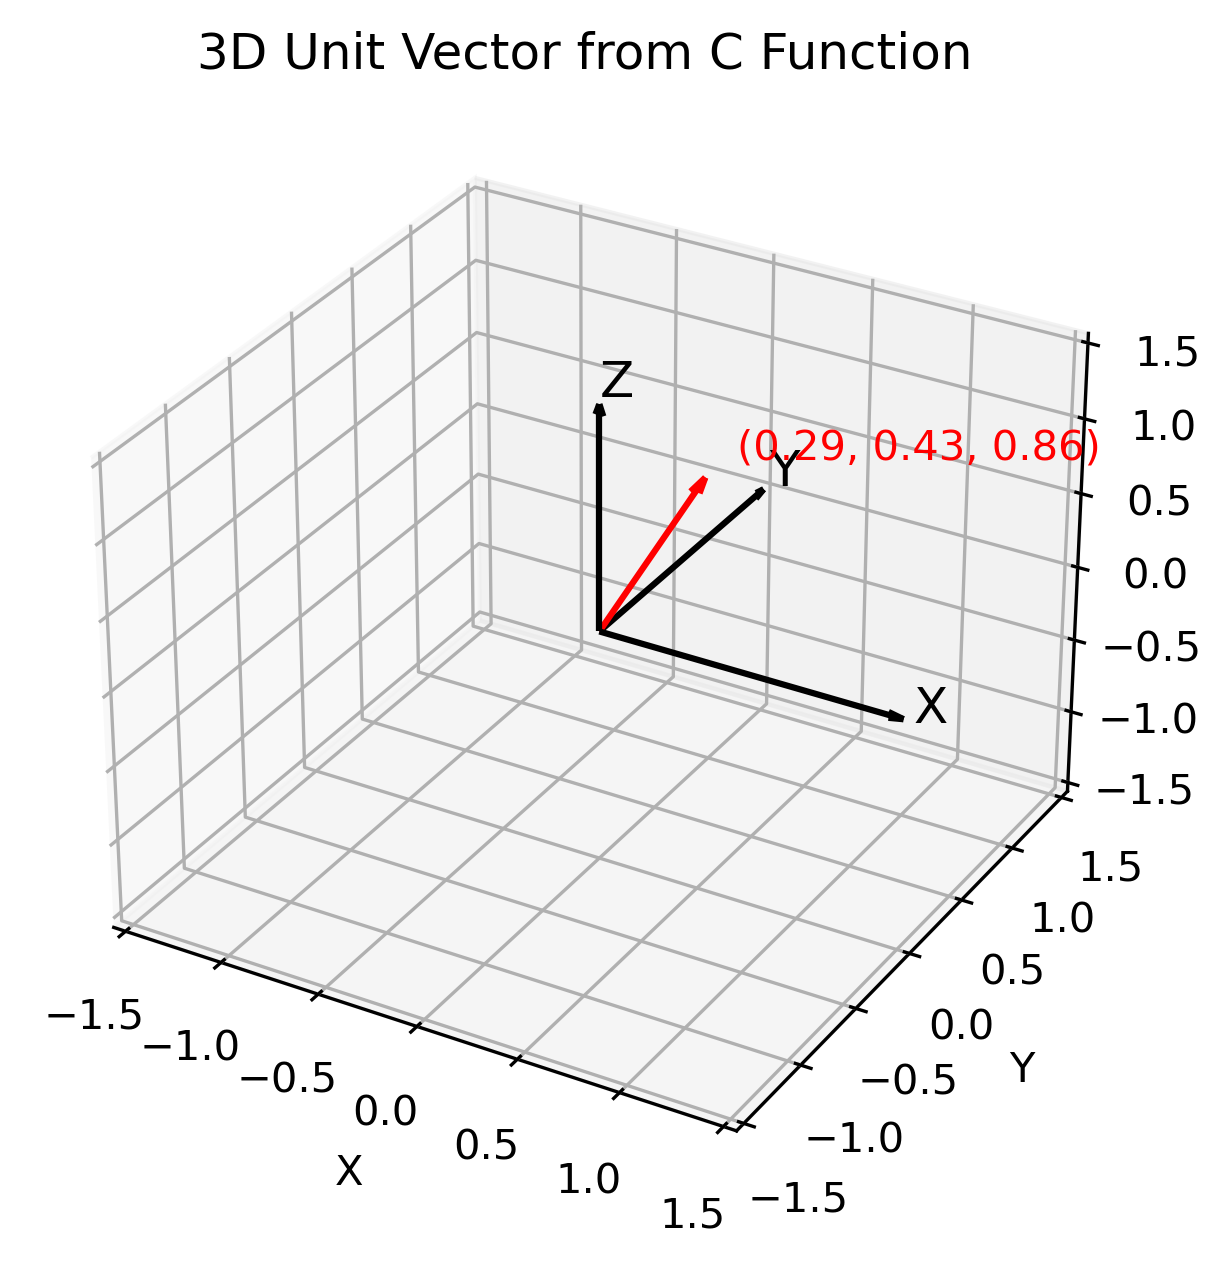
\includegraphics[width=0.52\linewidth]{figs/unit_vector3d}
	\caption{}
	\label{fig:unitvector3d}
\end{figure}
	

	
	
\end{document}